\documentclass{standalone}
\usepackage{tikz,amsmath}
\tikzset{block/.style = {draw, fill=white, very thick, rectangle, minimum height=1cm, minimum width=2cm},}
\tikzset{sum/.style= {draw, fill=white, very thick, circle, node distance=1cm},}
\begin{document}
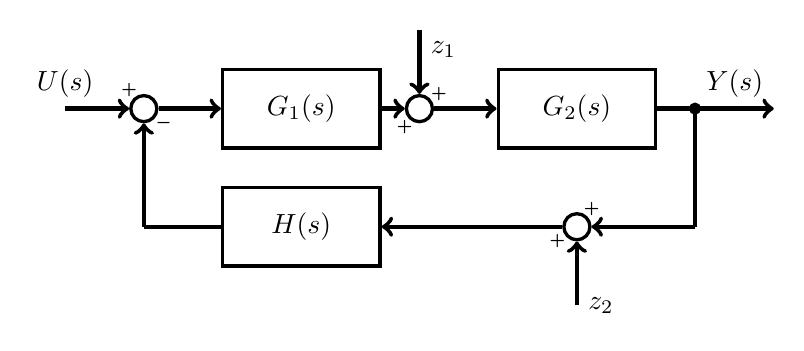
\begin{tikzpicture}[scale=2]
    \node[sum](sum)at(-1,0){};
    \node[sum](sum2)at(0.75,0){};
    \draw[->,ultra thick](-1.5,0)node[above]{$U(s)$}--(sum.180)node[above]{$\scriptscriptstyle\boldsymbol{+}$};


    \node[block, right of=sum, node distance=2cm](g){$G_1(s)$};
    \draw[->,ultra thick](sum.0)--(g.180);
    \draw[->,ultra thick](g.0)--(sum2.180)node[below]{$\scriptscriptstyle\boldsymbol{+}$};
    

    \filldraw[black](2.5,0)circle(1pt);


    \draw[->,ultra thick](0.75,0.5)node[below right]{$z_1$}--(sum2.90)node[right]{$\scriptscriptstyle\boldsymbol{+}$};

    \node[block]at(1.75,0)(k){$G_2(s)$};
    \draw[->,ultra thick](sum2.0)--(k.180);
    \draw[-,ultra thick](k.0)--(2.5,0);

    \draw[->,ultra thick](2.5,0)node[above right]{$Y(s)$}--(3,0);
    \draw[-,ultra thick](2.5,-0.75)--(2.5,0);

    \node[sum](sum3)at(1.75,-0.75){};
    \draw[->,ultra thick](2.5,-0.75)--(sum3.0)node[above]{$\scriptscriptstyle\boldsymbol{+}$};
    \draw[->,ultra thick](1.75,-1.25)node[right]{$z_2$}--(sum3.270)node[left]{$\scriptscriptstyle\boldsymbol{+}$};

    \node[block, below of=g, node distance=1.5cm](h){$H(s)$};
    \draw[->,ultra thick](sum3.180)--(h.0);
    \draw[-,ultra thick](h.180)--(-1,-0.75);

    \draw[->,ultra thick](-1,-0.75)--(sum.270)node[right]{$\scriptscriptstyle\boldsymbol{-}$};
\end{tikzpicture}
\end{document}